Reply proposed a workflow for the ETL process using Azure resources, as shown in figure \ref{fig:azure:workflow}.

Their proposal also included an architecture for performing analyses on the Data Warehouse.

\begin{figure}
    \centering
    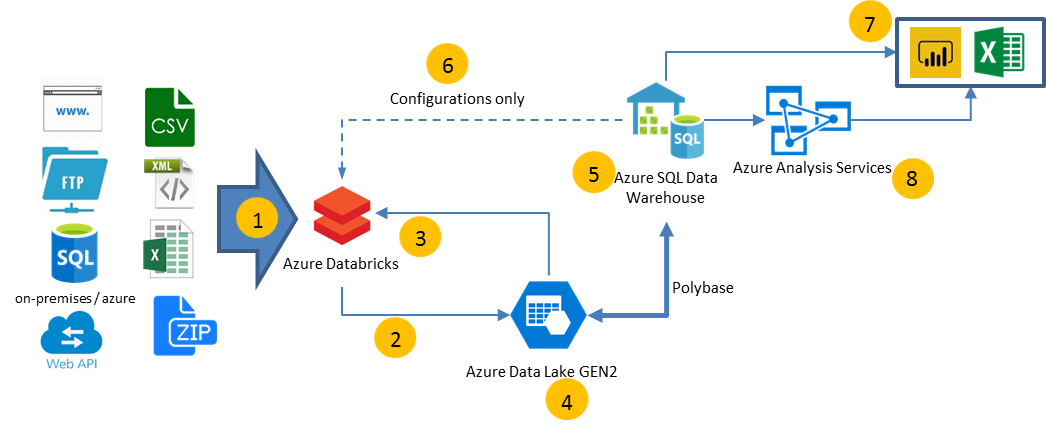
\includegraphics[width=\textwidth]{res/azure/workflow.png}
    \caption{Interaction between Azure components.}
    \label{fig:azure:workflow}
\end{figure}

\begin{enumerate}
    \item Data from several providers is downloaded by DataBricks in different ways, such as APIs, FTP or web scraping.
    \item This data is then stored on DataLake, under the \texttt{rawdata} folder.
    \item Those files are recovered by Databricks, which applies some transformations on the data, for example normalization or column removal.
    \item The result is saved again on DataLake, in \textit{csv} format, under the \texttt{srcdata} folder.
    \item The values from the \textit{csv} files are loaded into the data warehouse. The communication between the blob storage and the data warehouse is handled by Polybase.
    \item Some values stored in the data warehouse are accessed by Databricks and used as configuration settings.
    \item The data warehouse is queried by reporting tools, such as Excel or PowerBI, as well as algorithms developed by Axpo.
    \item In case of heavy workloads, it is also possible to query a copy of the data warehouse, located on Azure Analytics Services.
\end{enumerate}

